\section{Results}
Figure~\ref{fig:toroth} illustrates modelled monkeypox incidence and cumulative infections
in ``Toronto'' versus city~B under different vaccine allocation strategies.
Due to the larger population size,
greater epidemic potential ($R_0$), and
having all imported/seed cases in Toronto in this scenario,
allocating all 5000 vaccine doses to Toronto
yielded the fewest infections by day~120: 1630 (\subref{fig:inf.toroth.opt}). % MAN
Allocating vaccines proportionally to city size (\subref{fig:inf.toroth.prop}) yielded 1956 infections, % MAN
while no vaccination (\subref{fig:inf.toroth.none}) yielded 3466 infections. % MAN
\par
As shown in Figure~\ref{fig:inf.toroth.opt}, allocating most/all doses to one city (A)
allows incidence to rise exponentially in the other city (B).
However, this approach can still avert more infections overall over shorter time horizons,
after which more doses may become available.
Figure~\ref{fig:inf.default} illustrates the opposite case
(default model parameters in Table~\ref{tab:model.params}): two identical cities with equal seeding,
where the optimal allocation is equal between cities.
\begin{figure}[h]
  \begin{subfigure}{\linewidth}
    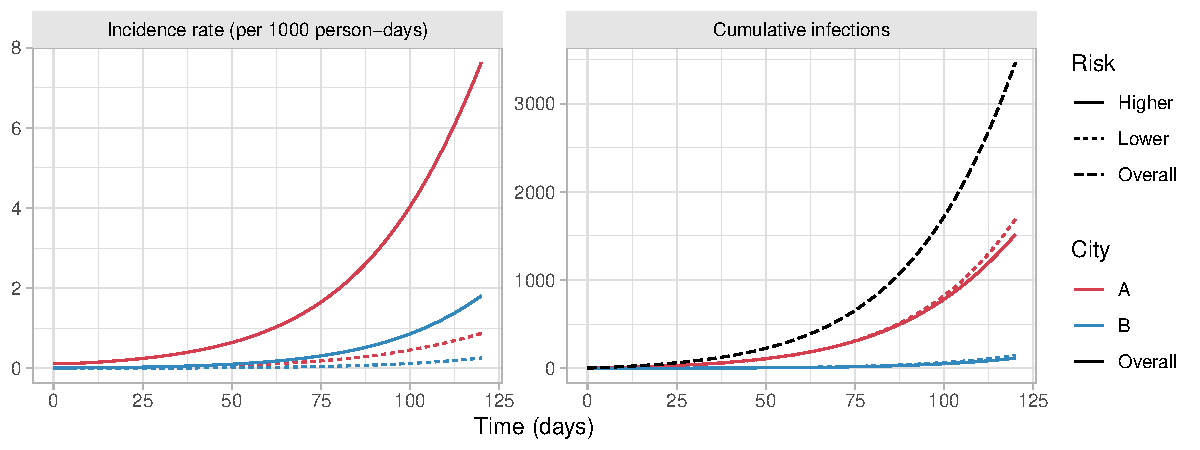
\includegraphics[width=\linewidth]{inf.toroth.none}
    \caption{No vaccination}
    \label{fig:inf.toroth.none}
  \end{subfigure}
  \begin{subfigure}{\linewidth}
    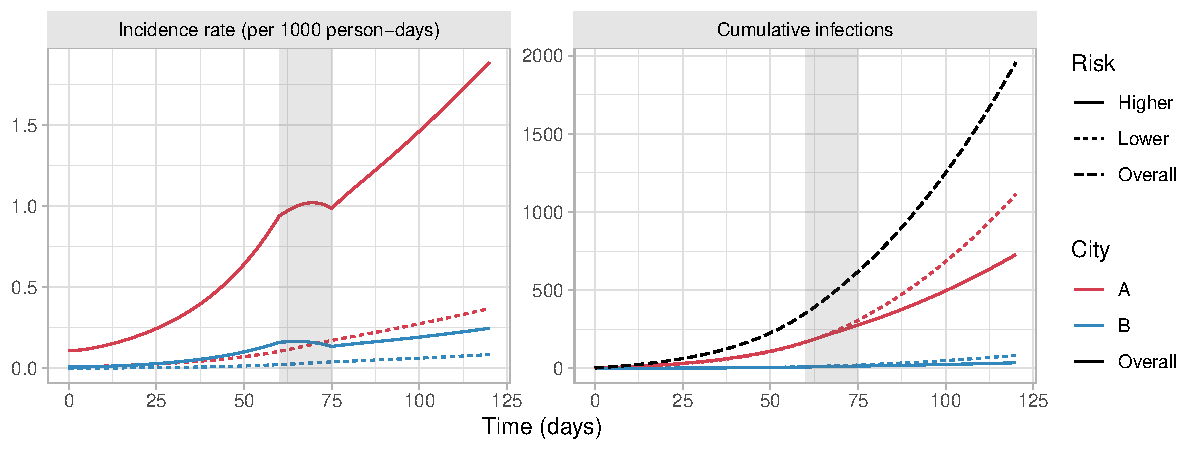
\includegraphics[width=\linewidth]{inf.toroth.prop}
    \caption{Proportional to city size: 75\% city~A, and 25\% city~B}
    \label{fig:inf.toroth.prop}
  \end{subfigure}
  \begin{subfigure}{\linewidth}
    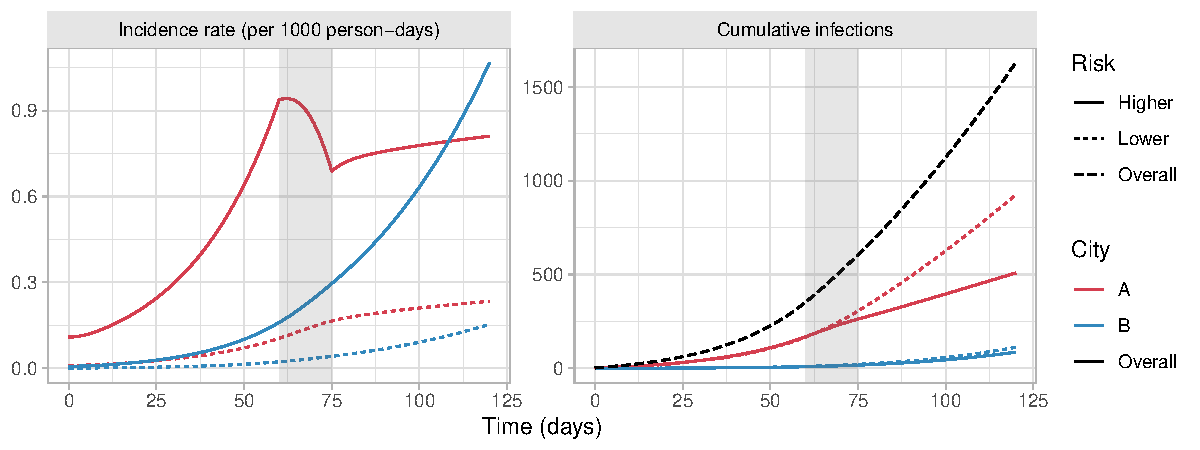
\includegraphics[width=\linewidth]{inf.toroth.opt}
    \caption{Optimal (most infections averted by day 120): 100\% city~A}
    \label{fig:inf.toroth.opt}
  \end{subfigure}
  \caption{Modelled monkeypox incidence and cumulative infections in two cities
    under two different vaccine allocation scenarios}
  \label{fig:toroth}
  \floatfoot
  Gray bar indicates period of vaccine roll-out (days 60--75).
  Cities loosely reflect Toronto and another medium-sized Ontario city.
\end{figure}
\par
Figure~\ref{fig:grid.opt} illustrates optimal vaccine allocation between cities A~and~B
across different epidemic conditions.
Figures~\ref{fig:grid.dci.none}--\ref{fig:grid.rdci.prop} further illustrate the
absolute and relative numbers of infections averted under optimal allocation
versus no vaccination (\ref{fig:grid.dci.none}--\ref{fig:grid.rdci.none}), and
versus vaccine allocation proportional to city size (\ref{fig:grid.dci.prop}--\ref{fig:grid.rdci.prop}).
Thus, Figures~\ref{fig:grid.dci.none}--\ref{fig:grid.rdci.prop}
show under what conditions optimal allocation is most important.
\par
The strongest determinants of optimal vaccine allocation were:
relative epidemic potential ($R_0$), share of seed cases, and city size;
though city size was proportional to
the size of the higher risk group under our modelling assumptions.
Thus, if a larger city had large $R_0$ and the majority of seed cases,
it was best to allocate most/all doses to that city in our analysis
(solid red/blue corners in Figure~\ref{fig:grid.opt}).
\par
For smaller cities with large $R_0$ and the majority of seed cases,
it was sometimes possible to vaccinate the entire higher risk group;
in this case, the remaining doses were best allocated to the other city,
yielding the plateaus (solid-colour triangles) in Figure~\ref{fig:grid.opt}:
(a,d,g) upper right; (c,f,i) lower left.
This plateau highlights how priority populations can change
if/after high levels of coverage are achieved in other populations.
\par
When cities with most/all seed cases had smaller $R_0$,
optimal allocation saw doses shared between cities (to varying degrees),
suggesting that both risk-based (reflecting $R_0$) and
proximity-based (reflecting initial cases) prioritization strategies
worked together to minimize transmission.
In such cases, the other city necessarily had few/no seed cases but larger $R_0$,
to which the same findings apply.
These conditions are represented by the yellow diagonal segments
in all facets of Figure~\ref{fig:grid.opt}.
\par
Finally, increased levels of mixing between cities
mainly acted to reduce the influence of initial seed cases,
and increase the influence of $R_0$
on optimal allocation of vaccines to each city;
this finding is visible in Figure~\ref{fig:grid.opt} as
stronger vertical gradients (contours are more horizontal) in (a,b,c) with more inter-city mixing, versus
stronger horizontal gradients (contours are more vertical) in (g,h,i) with less inter-city mixing.
\begin{figure}
  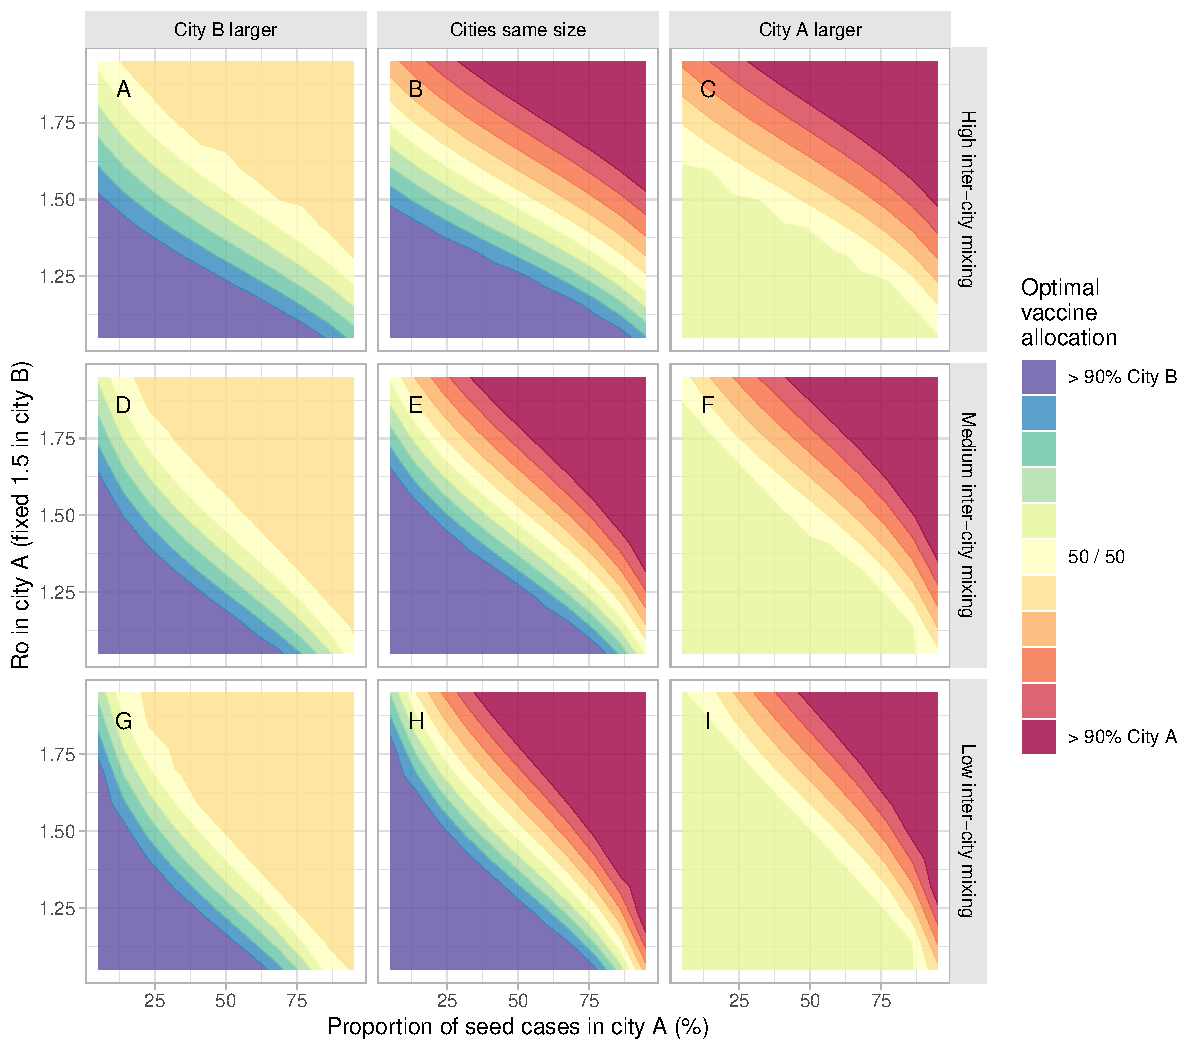
\includegraphics[width=\linewidth]{grid.opt.pdf}
  \caption{Optimal vaccine allocation between two cities under different epidemic conditions}
  \label{fig:grid.opt}
  \floatfoot
  \gridfoot
\end{figure}
